En esta sección, se presentan los resultados obtenidos al reproducir cada uno de
los experimentos de la sección anterior, es decir, los experimentos que los autores
presentan en su trabajo \cite{jsantos-amonteagudo-1-2014}.

Antes de todo, hay que tener en cuenta la componente aleatoria de la simulación. Esto es, por
la realización de sorteos de cara a ejecutar la mitosis u otra acción. En consecuencia, la aparición
de un marcador u otro, como se verá a continuación, provoca alteraciones en la simulación, de modo que
el comportamiento puede variar. En este caso, lo que se pretende es llegar a la misma conclusión que los autores,
por tanto, el análisis de los resultados propios debe hacerse con ese objetivo en mente.

\section{Influencia del parámetro \textit{Tasa de mutación base (m)}}

Las células de la simulación, y como se ha descrito en secciones previas, tienen asociado una propiedad que está relacionada con la aparición
de nuevas mutaciones durante la mitosis, este es, el parámetro \textit{tasa de mutación base} o $m$. En este experimento,
se pretende someter a la simulación a diferentes configuraciones de este parametros para estudiar qué
progresión presentan los tumores.

Se parte de una probabilidad de aparición de mutaciones baja, ya que, el sorteo se efectúa con una probabilidad de
$1/m$, por lo que, a mayor valor del parámetro $m$, menor probabilidad de que ocurra. En este caso, se
realizan tres simulaciones, para $m=10.000$, $m=1.000$ y $m=100$.

\subsection{Experimento 1: Tasa de mutación base igual a 10.000}

En la primera de las tres figuras, la figura~\ref{fig:ownexp1-1}, se presenta el resultado
de la simulación desde el punto de vista de las células sanas y las células cancerosas.

\begin{figure}[h]
\centering
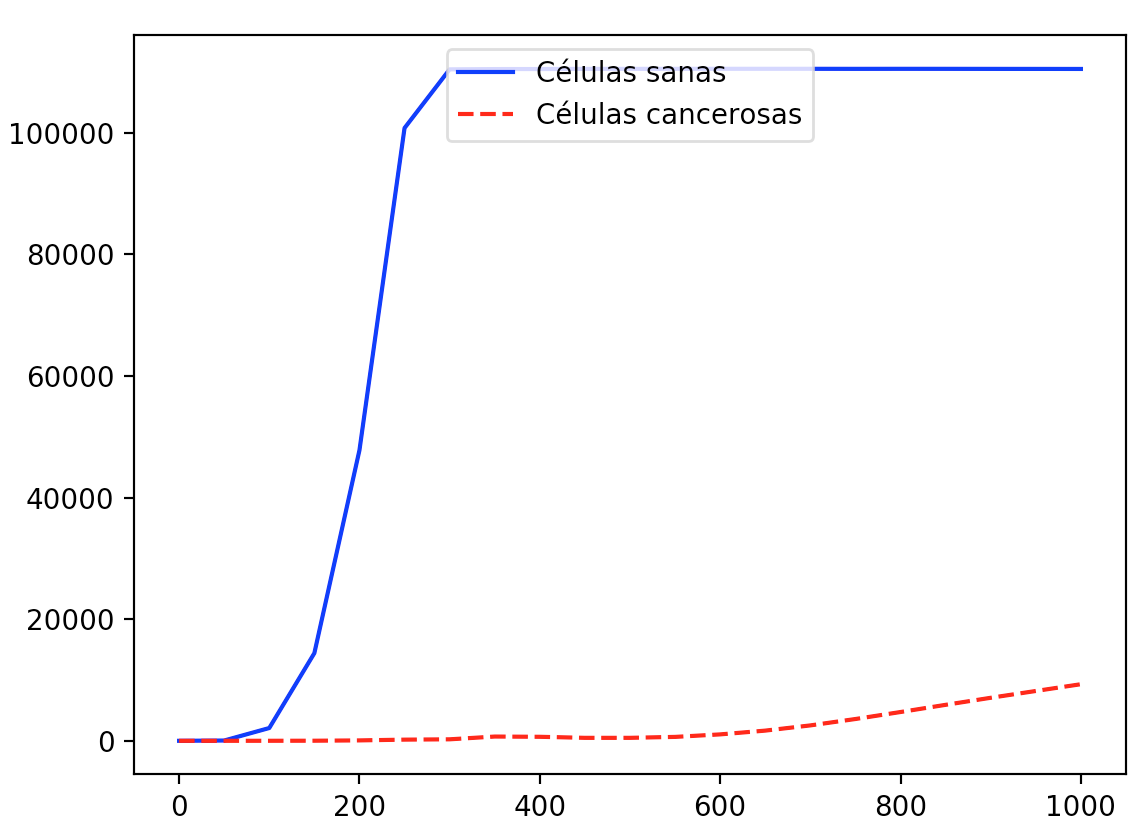
\includegraphics[scale=0.6]{figures/experiments/exp1/healthvscarcino}
\caption{Células sanas frente a células cancerosas como resultado de la simulación para el experimento con $m = 10.000$.}
\label{fig:ownexp1-1}
\end{figure}

El resultado obtenido es bastante similar, por lo que se debe observar la evolución de los
marcadores, la cual se presenta en la figura~\ref{fig:ownexp1-2}. En este caso, el marcador
más relevante es $SG$. Aunque, en este caso, se ha asociado a la mutación $EI$, el comportamiento
global se debe al marcador $SG$. Es decir, el tumor crece por la parte exterior de la rejilla que,
como se ha descrito en el capítulo anterior, se debe a un menor factor de crecimiento. El marcador
$EI$ surge en una de esas células y evoluciona sin alterar el comportamiento global.

\begin{figure}[h]
\centering
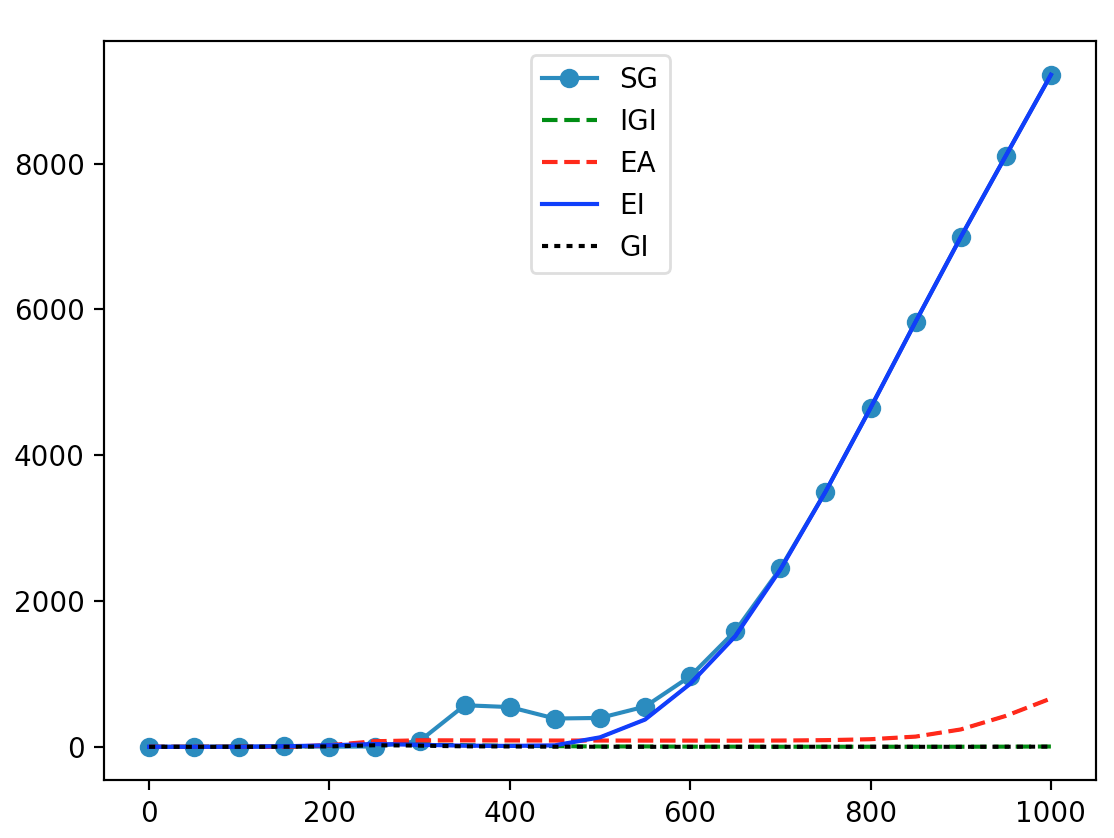
\includegraphics[scale=0.6]{figures/experiments/exp1/mutations}
\caption{Evolución de los marcadores como resultado de la simulación para el experimento con $m = 10.000$.}
\label{fig:ownexp1-2}
\end{figure}

En una vista de la rejilla, como en la~\ref{fig:ownexp1-3}, se puede observar como
efectivamente tiende a ocupar el exterior, lo que coincide con los resultados obtenidos por los
autores.

\begin{figure}[h]
\centering
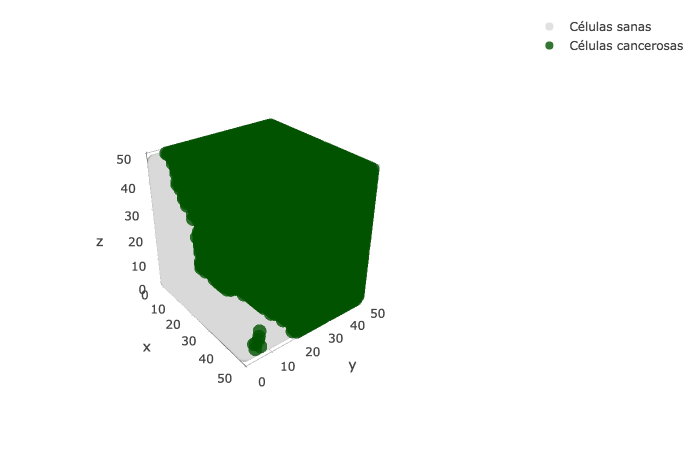
\includegraphics[scale=0.6]{figures/experiments/exp1/grid}
\caption{Rejilla resultante de la simulación para el experimento con $m = 10.000$.}
\label{fig:ownexp1-3}
\end{figure}

\subsection{Experimento 2: Tasa de mutación base igual a 1.000}

En la primera de las tres figuras, la figura~\ref{fig:ownexp2-1}, se presenta el resultado
de la simulación desde el punto de vista de las células sanas y las células cancerosas,
pero en esta ocasión con el parámetro establecido a $m=1.000$.

\begin{figure}[h]
\centering
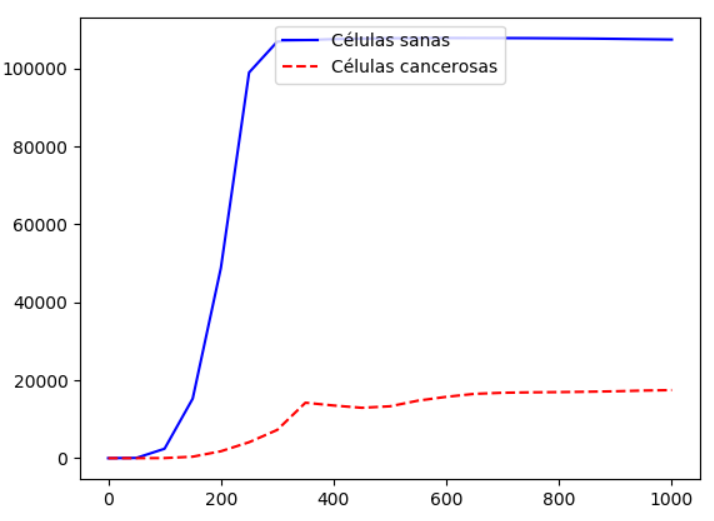
\includegraphics[scale=0.8]{figures/experiments/exp2/healthvscarcino}
\caption{Células sanas frente a células cancerosas como resultado de la simulación para el experimento con $m = 1.000$.}
\label{fig:ownexp2-1}
\end{figure}

El resultado obtenido es bastante similar, por lo que se debe observar la evolución de los
marcadores, la cual se presenta en la figura~\ref{fig:ownexp2-2}. En este caso, el marcador
más relevante es $SG$. Aunque, en este caso, se ha asociado también a la mutación $EI$. El segundo marcador
más relevante tras $SG$, es el marcador $EA$. Este comportamiento se observa también en
los resultados obtenidos por los autores.

\begin{figure}[h]
\centering
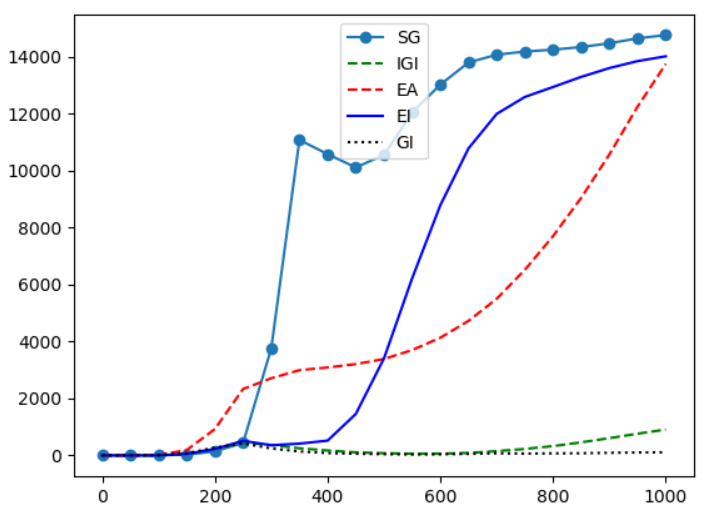
\includegraphics[scale=0.8]{figures/experiments/exp2/mutations}
\caption{Evolución de los marcadores como resultado de la simulación para el experimento con $m = 1.000$.}
\label{fig:ownexp2-2}
\end{figure}

En una vista de la rejilla, como en la~\ref{fig:ownexp2-3}, se puede observar como
tiende a ocupar el exterior y, en este caso, también una pequeña parte del espacion
interior de la rejilla, lo que coincide con los resultados obtenidos por los
autores.

\begin{figure}[h]
\centering
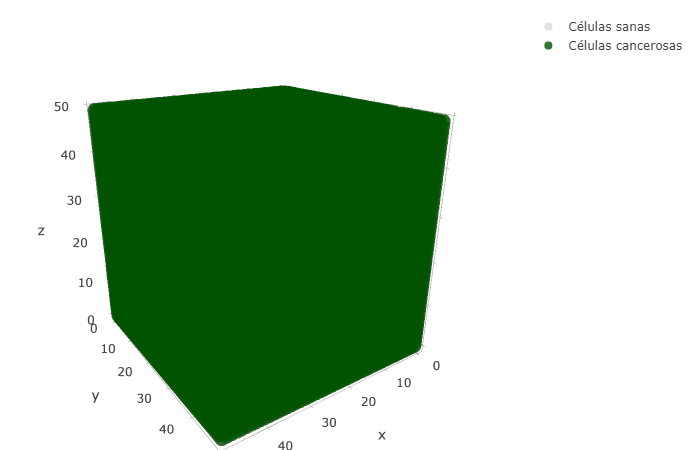
\includegraphics[scale=0.6]{figures/experiments/exp2/grid}
\caption{Rejilla resultante de la simulación para el experimento con $m = 10.000$.}
\label{fig:ownexp2-3}
\end{figure}

\subsection{Experimento 3: Tasa de mutación base igual a 100}

En la primera de las tres figuras, la figura~\ref{fig:ownexp3-1}, se presenta el resultado
de la simulación desde el punto de vista de las células sanas y las células cancerosas,
pero en esta ocasión con el parámetro establecido a $m=100$.

\begin{figure}[h]
\centering
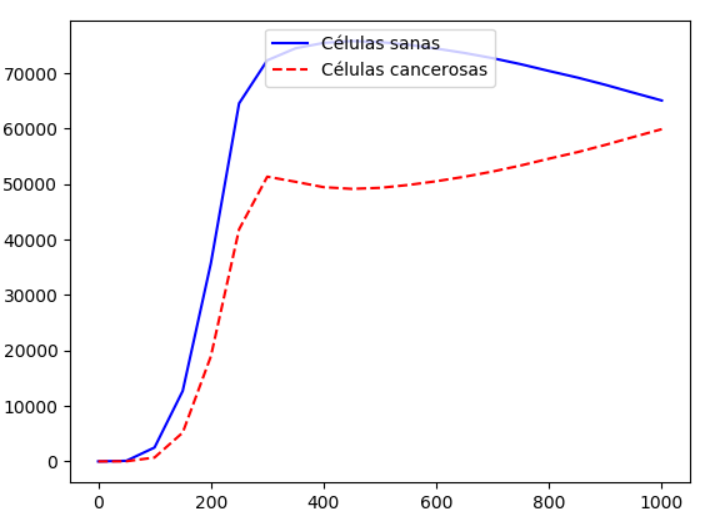
\includegraphics[scale=0.8]{figures/experiments/exp3/healthvscarcino}
\caption{Células sanas frente a células cancerosas como resultado de la simulación para el experimento con $m = 100$.}
\label{fig:ownexp3-1}
\end{figure}

El resultado obtenido aquí es difernte a priori. El número de células cancerosas
no supera rápidamente al de células sanas, por el contrario, al final de la simulación
se observa como si hubiera más iteraciones pronto llegarían a representar la inmensa
totalidad de la rejilla.

Esto se explica por la evolución de los marcadores de dicha simulación, como se muestra en
la figura~\ref{fig:ownexp3-2}. El marcador $EA$ presenta un comportamiento similar, pero
no es suficiente por sí solo. En este caso, la menor presencia del marcador $IGI$, el cual
permite superar el límite de la falta de espacio que tiene lugar en la zona interior de la rejilla,
provoca que no superen en número las células cancerosas a las sanas.

\begin{figure}[h]
\centering
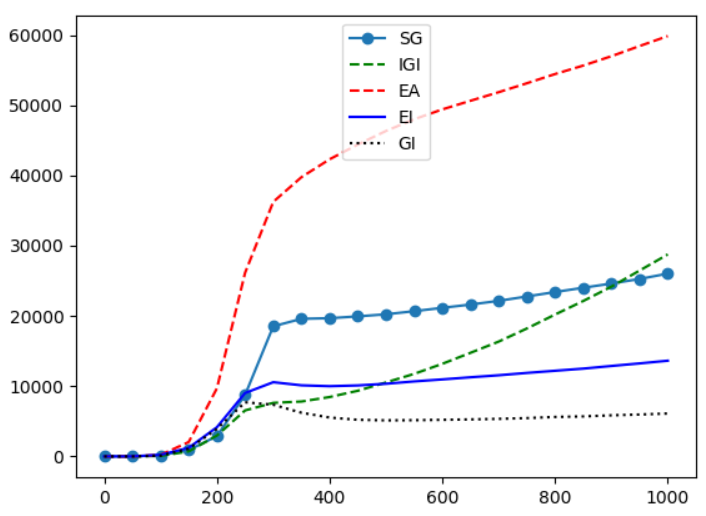
\includegraphics[scale=0.8]{figures/experiments/exp3/mutations}
\caption{Evolución de los marcadores como resultado de la simulación para el experimento con $m = 100$.}
\label{fig:ownexp3-2}
\end{figure}

Aunque, desde el punto de vista de la rejilla, como se muestra en la figura~\ref{fig:ownexp3-2},
el comportamiento es parecido salvando los detalles comentados anteriormente. Es decir,
hay mayor presencia de células cancerosas en la zona interior.

\begin{figure}[h]
\centering
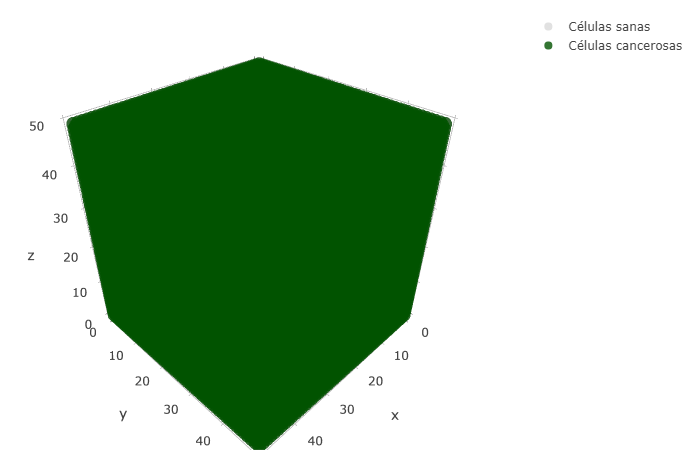
\includegraphics[scale=0.6]{figures/experiments/exp3/grid}
\caption{Rejilla resultante de la simulación para el experimento con $m = 100$.}
\label{fig:ownexp3-3}
\end{figure}

\section{Influencia del resto de parámetros}

Los autores realizan un segundo experimento con el objetivo de observar los efectos
que tienen el resto de parámetros sobre la simulación. Para ello, varían los parámetros de
la simulación, como se puede observar en la siguiente tabla:

\begin{table}[h!]
  \centering
  \caption{Valores de los parámetros.}
  \label{tab:table1}
  \begin{tabular}{ccc}
    \toprule
    Nombre & Símbolo & Valor\\
    \midrule
    Tasa de mutación base & m & 100.000\\
    Tamaño del telómero & tl & 35\\
    Muerte por daño genético & e & 20\\
    Factor de incremento de tasa de mutación base & i & 100\\
    Muerte de un vecino & g & 10\\
    Muerte aleatoria & a & 400\\
    \bottomrule
  \end{tabular}
\end{table}

Los resultados obtenidos se muestran a continuación.

\begin{figure}[h]
\centering
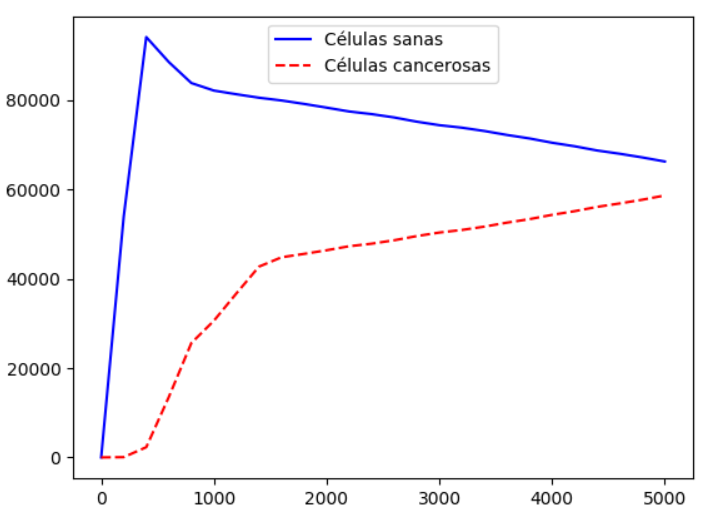
\includegraphics[scale=0.8]{figures/experiments/exp4/healthvscarcino}
\caption{Células sanas frente a células cancerosas como resultado de la simulación para el experimento con $m = 100.000$.}
\end{figure}

\begin{figure}[h]
\centering
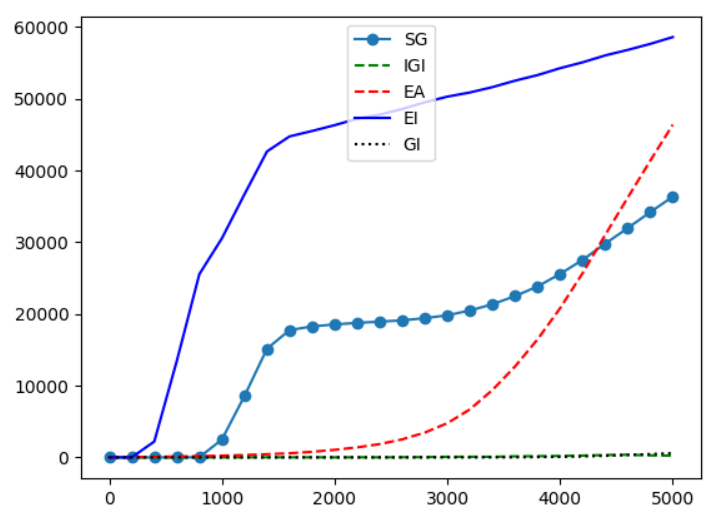
\includegraphics[scale=0.8]{figures/experiments/exp4/mutations}
\caption{Evolución de los marcadores como resultado de la simulación para el experimento con $m = 100.000$.}
\end{figure}

\begin{figure}[h]
\centering
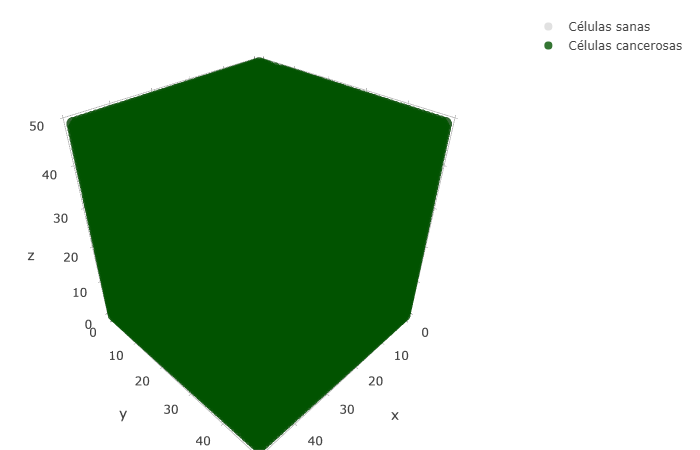
\includegraphics[scale=0.6]{figures/experiments/exp4/grid}
\caption{Rejilla resultante de la simulación para el experimento con $m = 100.000$.}
\end{figure}

\section{Influencia de parámetros con rejilla completa de células sanas}

\begin{figure}[h]
\centering
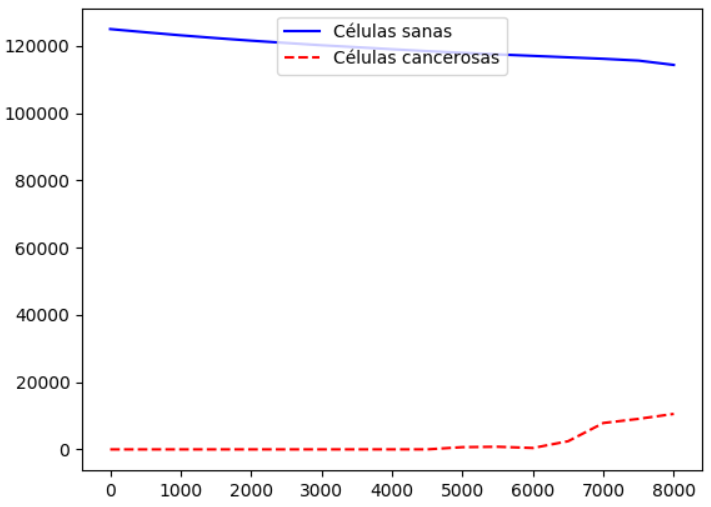
\includegraphics[scale=0.8]{figures/experiments/exp5/healthvscarcino}
\caption{Evolución de las células sanas frente a células cancerosas con rejilla completa de células sanas y parámetros por defecto.}
\end{figure}

\begin{figure}[h]
\centering
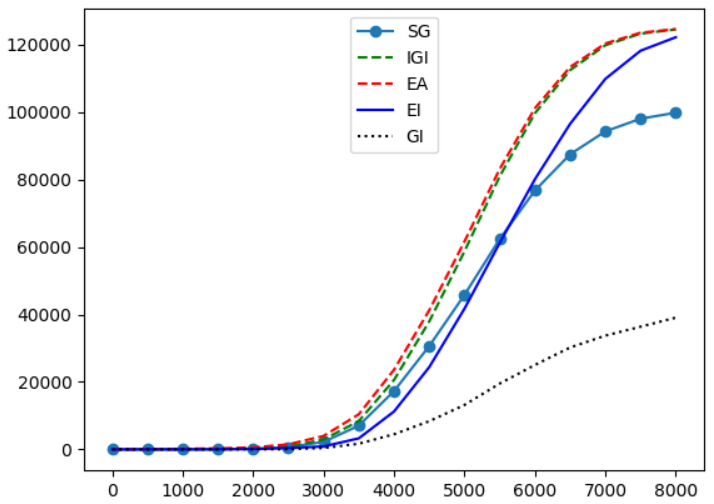
\includegraphics[scale=0.8]{figures/experiments/exp5/mutations}
\caption{Evolución de los marcadores cancerosos con rejilla completa de células sanas y parámetros por defecto.}
\end{figure}

\begin{figure}[h]
\centering
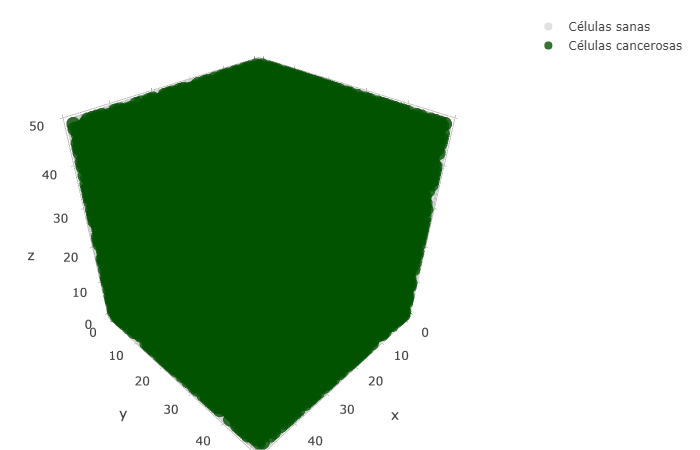
\includegraphics[scale=0.6]{figures/experiments/exp5/grid}
\caption{Rejilla resultante de la simulación iniciada completa de células sanas.}
\end{figure}

\section{Relevancia de los marcadores}

\begin{figure}[h]
\centering
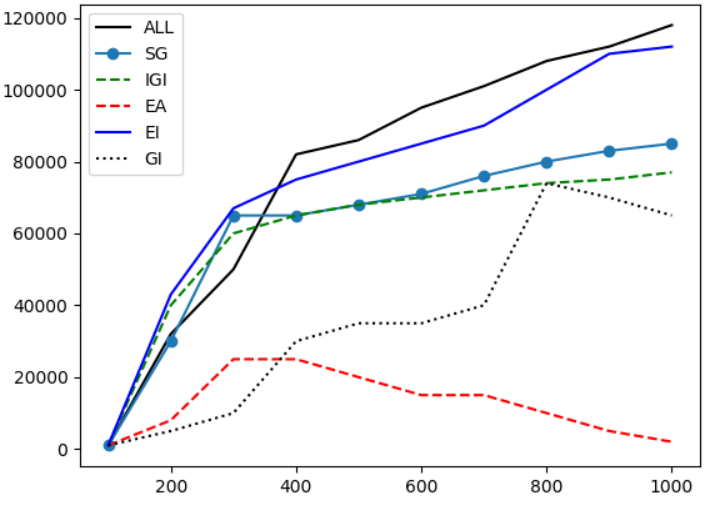
\includegraphics[scale=0.8]{figures/experiments/exp7/exp7-1}
\caption{Efecto de la eliminación de un marcador con parámetros por defecto excpeto con $m = 100$.}
\end{figure}

\begin{figure}[h]
\centering
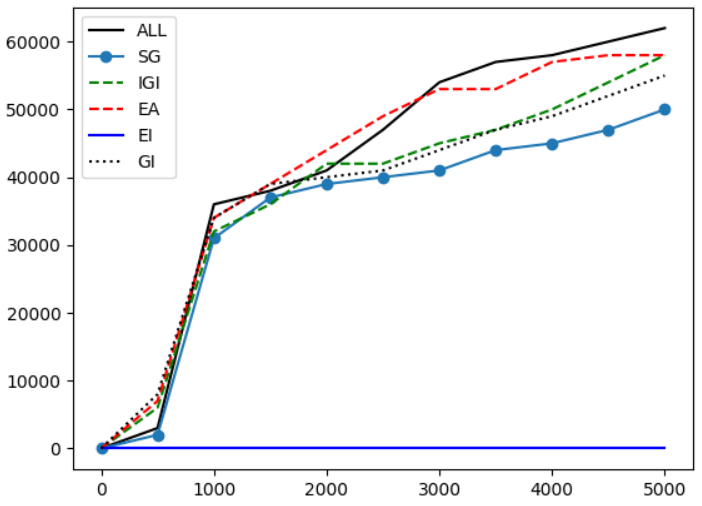
\includegraphics[scale=0.6]{figures/experiments/exp7/exp7-2}
\caption{Efecto de la eliminación de un marcador con parámetros del cuadro 7.1.}
\end{figure}
